% !TeX program = lualatex

\documentclass[12pt, a4paper]{article}

\usepackage[T1]{fontenc}
\usepackage{times}

\usepackage{amsmath, amssymb}
\usepackage{mathshorthand}

\usepackage[lite, zswash, subscriptcorrection, straightbraces]{mtpro2}
\DeclareMathSymbol{0}{\mathalpha}{operators}{`0}
\DeclareMathSymbol{1}{\mathalpha}{operators}{`1}
\DeclareMathSymbol{2}{\mathalpha}{operators}{`2}
\DeclareMathSymbol{3}{\mathalpha}{operators}{`3}
\DeclareMathSymbol{4}{\mathalpha}{operators}{`4}
\DeclareMathSymbol{5}{\mathalpha}{operators}{`5}
\DeclareMathSymbol{6}{\mathalpha}{operators}{`6}
\DeclareMathSymbol{7}{\mathalpha}{operators}{`7}
\DeclareMathSymbol{8}{\mathalpha}{operators}{`8}
\DeclareMathSymbol{9}{\mathalpha}{operators}{`9}

\usepackage{tikz}
\usetikzlibrary{decorations.markings, arrows.meta, calc}

\tikzset{
	shorten >= 3,
	tri/.tip={Triangle[angle=25:8pt]}, 
	dashed/.style={dash pattern=on 5pt off 3pt},
	% 1. Single arrow at position (default is 0.5)
	arrow at/.style={
		postaction={
			decorate,
			decoration={
				markings,
				mark=at position #1 with {\arrow[scale=1.3]{tri}}
			}
		}
	},
	arrow at/.default=0.5,
	%
	% 2. Custom arrow (2 arguments: position and style options)
	arrow style/.style 2 args={
		postaction={
			decorate,
			decoration={
				markings,
				mark=at position #1 with {\arrow[#2]{tri}}
			}
		}
	},
	%
	% 3. Repeated arrows (3 arguments: start, end, step) -> Use "style n args={3}"
	arrows step/.style n args={3}{
		postaction={
			decorate,
			decoration={
				markings,
				mark=between positions #1 and #2 step #3 with {\arrow[scale=1.2]{tri}}
			}
		}
	}
}

\begin{document}
	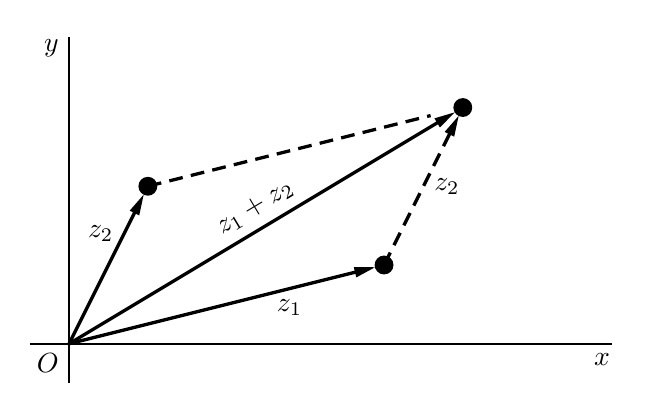
\begin{tikzpicture}[thick]
		% Axes
		\draw (-0.5,0) -- (7,0) node[below left] {$x$};
		\draw (0,-0.5) -- (0,4) node[below left] {$y$};
		
		\coordinate (O) at (0, 0) node[below left] {$O$};
		\coordinate (z2) at (1, 2);
		\coordinate (z1) at (4, 1);
		\coordinate (z1plusz2) at ($(z1) + (z2)$);
		
		\foreach \x in {z1, z2, z1plusz2}{\draw[fill=black] (\x) circle (3pt);}
		\draw[-tri, very thick] (O) -- (z1) node[pos=0.7, below]{$z_1$};
		\draw[-tri, very thick] (O) -- (z2) node[pos=0.7, left]{$z_2$};
		\draw[-tri, very thick] (O) -- (z1plusz2) node[pos=0.5, sloped, above]{$z_1 + z_2$};
		\draw[-tri, very thick, dashed] (z1) -- (z1plusz2) node[pos=0.5, right]{$z_2$};
		\draw[dashed, very thick, shorten >= 12] (z2) -- (z1plusz2) ;
	\end{tikzpicture}

	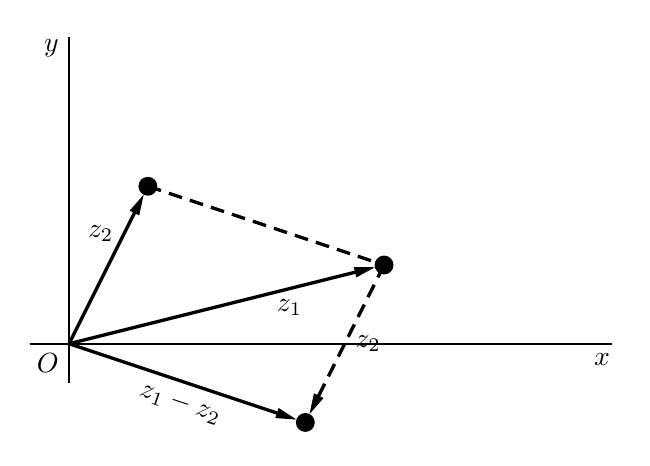
\begin{tikzpicture}[thick]
	% Axes
	\draw (-0.5,0) -- (7,0) node[below left] {$x$};
	\draw (0,-0.5) -- (0,4) node[below left] {$y$};
	
	\coordinate (O) at (0, 0) node[below left] {$O$};
	\coordinate (z2) at (1, 2);
	\coordinate (z1) at (4, 1);
	\coordinate (z1plusz2) at ($(z1) - (z2)$);
	
	\foreach \x in {z1, z2, z1plusz2}{\draw[fill=black] (\x) circle (3pt);}
	\draw[-tri, very thick] (O) -- (z1) node[pos=0.7, below]{$z_1$};
	\draw[-tri, very thick] (O) -- (z2) node[pos=0.7, left]{$z_2$};
	\draw[-tri, very thick] (O) -- (z1plusz2) node[pos=0.5, sloped, below]{$z_1 - z_2$};
	\draw[-tri, very thick, dashed] (z1) -- (z1plusz2) node[pos=0.5, right]{$z_2$};
	\draw[dashed, very thick] (z2) -- (z1) ;
\end{tikzpicture}
\end{document}